\begin{frame}
  \frametitle{\textbf{Flow in HI Collisions}}
  \begin{columns}
    \column{0.5\textwidth}
    \begin{itemize}
    \item QGP is often modeled as a \textbf{hydrodynamic fluid} $\to$ initial spacial anisotropies result in momentum-space anisotropies
    \item Flow harmonics $v_n$ $\to$ quantify the $\phi$-space anisotropy
    \end{itemize}
    \begin{align*}
      \cfrac{dN}{d\phi} = A \cdot \left( 1 + 2\sum_{n = 1}^{\infty} v_n \cos\left[n(\phi - \bar{\Psi}_{n})\right]   \right) 
    \end{align*}
    \begin{itemize}
    \item $v_2$ is most closely correlated with the initial-state geometry
    \item $v_2$ scales with parton number $\to$ flow is contributed on the parton level   $\to$ \textbf{evidence of deconfinement}
    \item Hydrodynamic models $\to$ QGP is a near \textit{perfect fluid}
    \end{itemize}
    \column{0.4\textwidth}
    \only<1>{
      \centering
      
      \begin{tikzpicture}
        \node{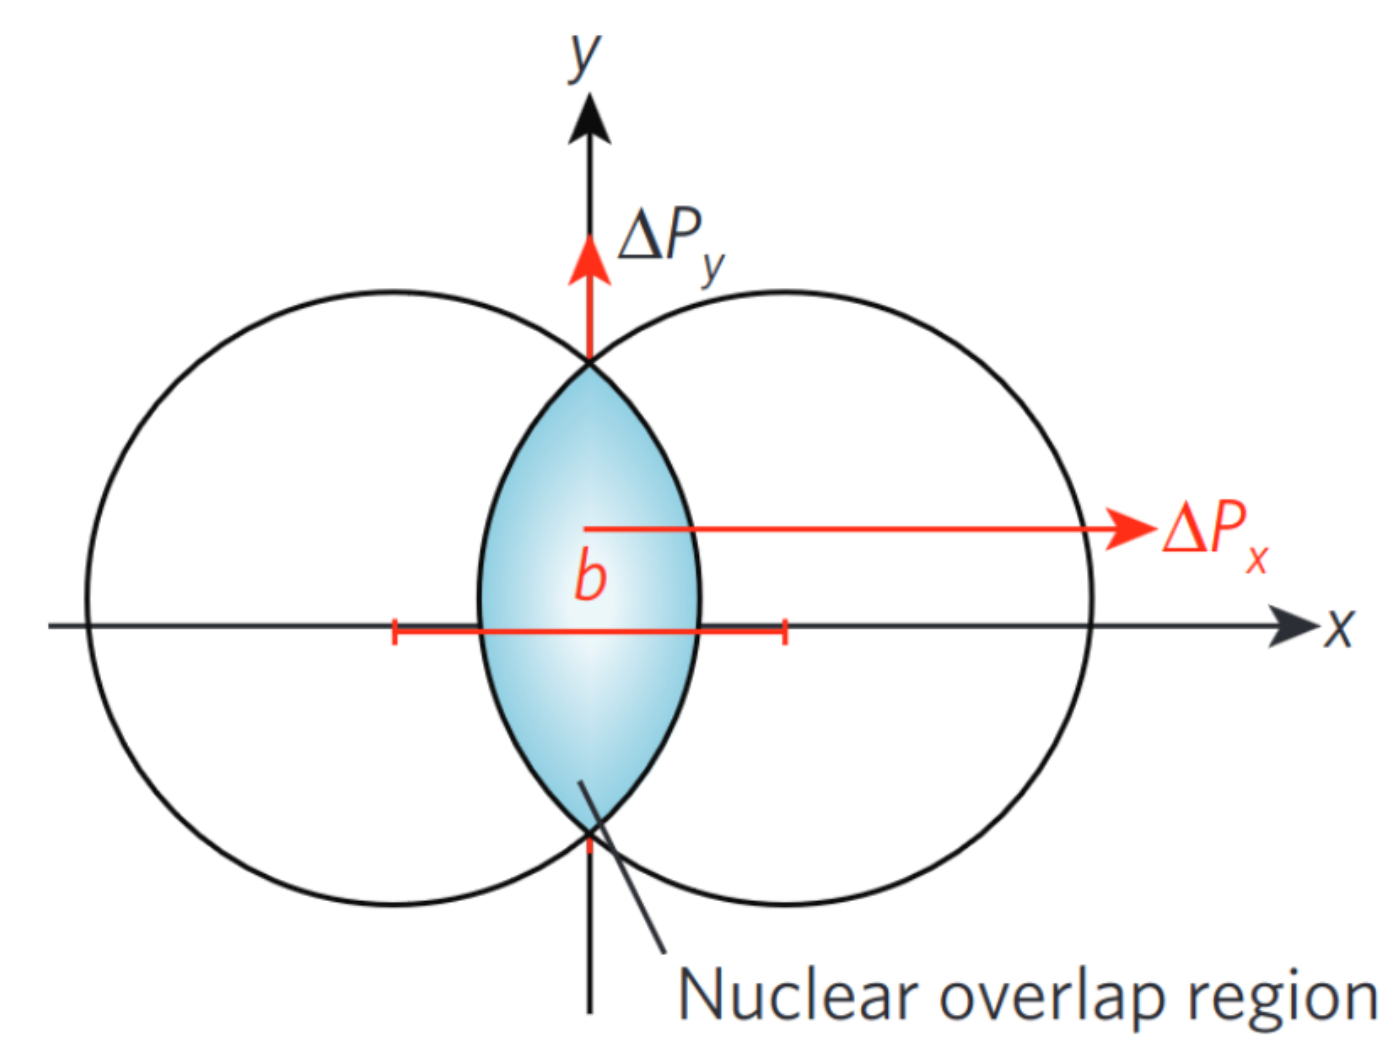
\includegraphics[width=0.8\textwidth]{nuclear-overlap-region-crop.png}};
      \end{tikzpicture}

      \
      
      \begin{tikzpicture}
        \node{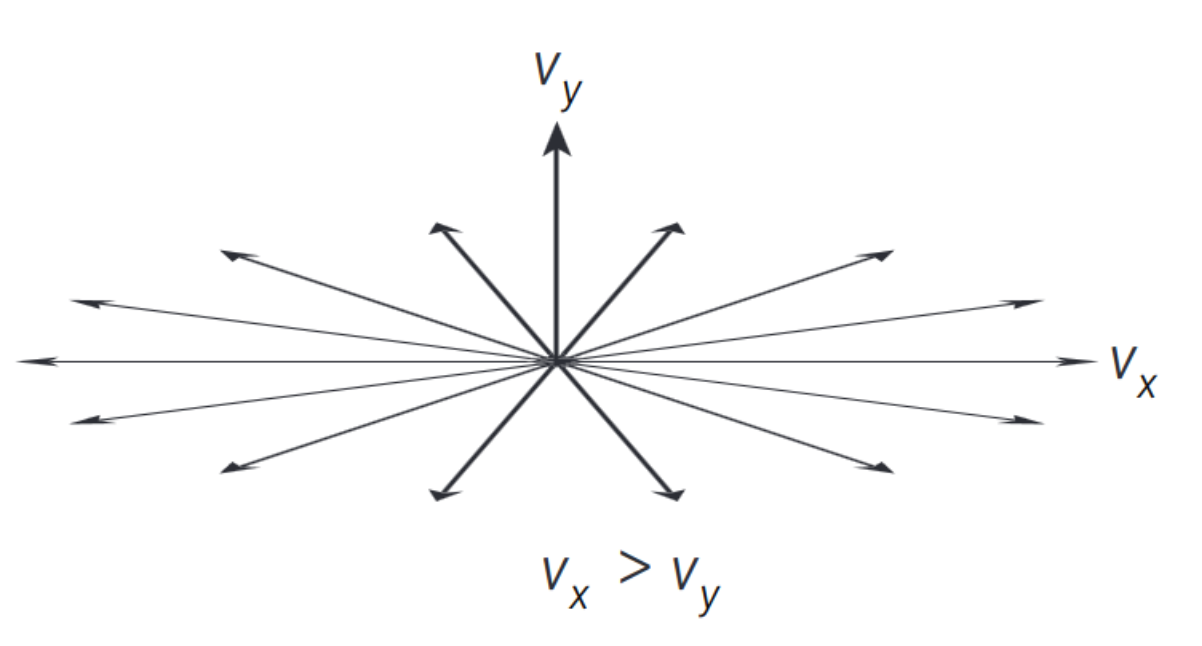
\includegraphics[width=0.8\textwidth]{velocity-anisotropy.png}};
        \node[font=\tiny] at (1.5,-1) {\href{https://arxiv.org/abs/1802.04801}{arXiv:1802.04801}};
      \end{tikzpicture}

      \

      
      \begin{tikzpicture}
        \node{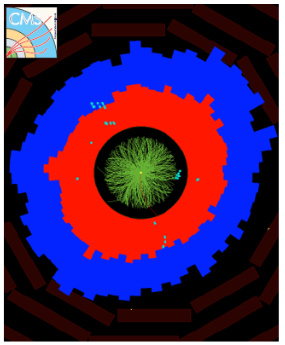
\includegraphics[width=0.35\textwidth]{asymmetric-event-display.png}};
      \end{tikzpicture}

      
    }

    \only<2>{
      \centering
      \begin{tikzpicture}
        \node{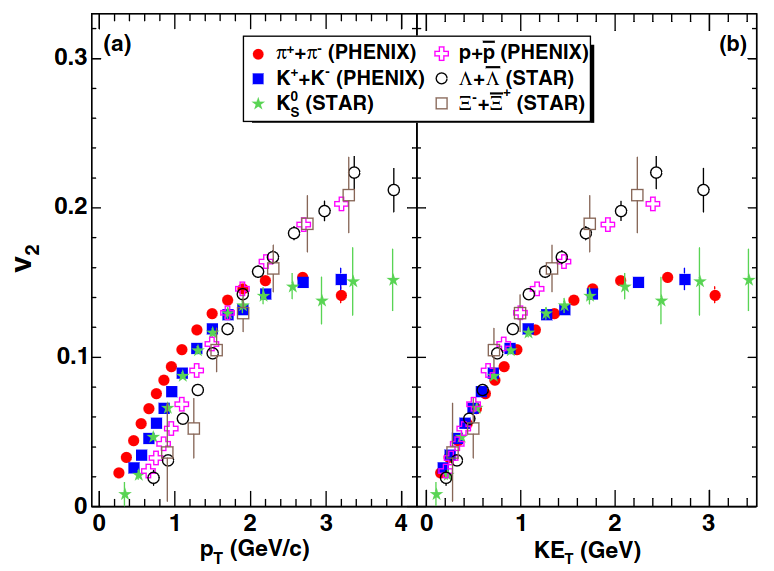
\includegraphics[width=\textwidth]{v2-before-scaling.png}};
        \node[font=\tiny,align=left] at (-1,0.5) {\textbf{baryons}};
        \node[font=\tiny,align=left] at (-0.3,-0.4) {\textbf{mesons}};
        \node[font=\tiny,align=left] at (1.0,0.5) {\textbf{baryons}};
        \node[font=\tiny,align=left] at (1.7,-0.4) {\textbf{mesons}};
        \node[font=\tiny] at (1.3,1.9) {\href{https://journals.aps.org/prl/abstract/10.1103/PhysRevLett.98.162301}{Phys. Rev. Lett. 98, 162301}};
      \end{tikzpicture}

      \
      
      \begin{tikzpicture}
        \node{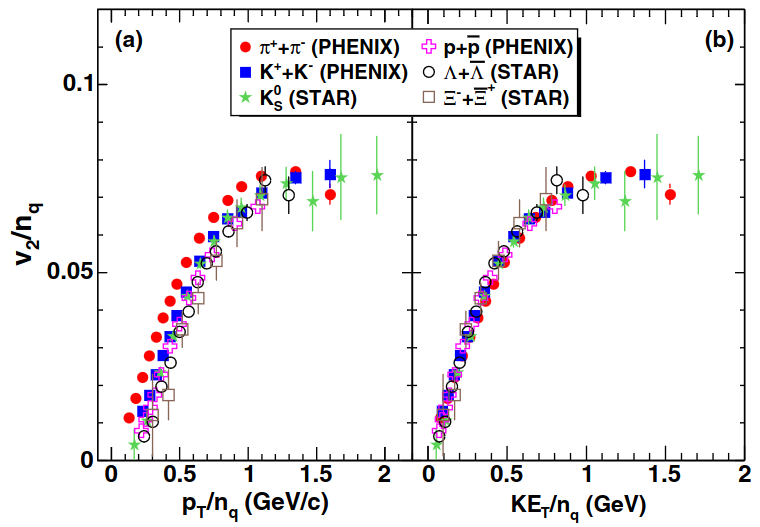
\includegraphics[width=\textwidth]{v2-after-scaling.png}};
      \end{tikzpicture}
      
    }
    

    
  \end{columns}
    
\end{frame}
